\documentclass[a4paper,12pt]{article}



%%% Работа с русским языком
% кодировка
\usepackage[utf8]{inputenc} 
\usepackage[T2A]{fontenc}	
\usepackage[english,russian]{babel}   %% загружает пакет многоязыковой вёрстки
\usepackage{cmap}
\usepackage{algorithm}
\usepackage{algorithmic} 
\usepackage{indentfirst}
\usepackage{xcolor}
\usepackage{hyperref}

% Цвета для гиперссылок
\definecolor{linkcolor}{HTML}{799B03} % цвет ссылок
\definecolor{urlcolor}{HTML}{799B03} % цвет гиперссылок

\hypersetup{pdfstartview=FitH,  linkcolor=linkcolor,urlcolor=urlcolor, colorlinks=true}
%%% Дополнительная работа с математикой
\usepackage{amsmath,amsfonts,amssymb,amsthm,mathtools} % AMS
\usepackage{amsfonts}
\usepackage[miktex]{gnuplottex} % <- Use instead if running TeX Live.

\usepackage{icomma} % "Умная" запятая: $0,2$ --- число, $0, 2$ --- перечисление
%% Номера формул
%\mathtoolsset{showonlyrefs=true} % Показывать номера только у тех формул, на которые есть \eqref{} в тексте.
%\usepackage{leqno} % Нумерация формул слева

%% Свои команды
\DeclareMathOperator{\sgn}{\mathop{sgn}}

%% Перенос знаков в формулах (по Львовскому)
\newcommand*{\hm}[1]{#1\nobreak\discretionary{}
	{\hbox{$\mathsurround=0pt #1$}}{}}

%%% Работа с картинками
\usepackage{graphicx}  % Для вставки рисунков
\usepackage{calc}
\usepackage{subcaption}
\graphicspath{{images/}{images2/}}  % папки с картинками
\setlength\fboxsep{3pt} % Отступ рамки \fbox{} от рисунка
\setlength\fboxrule{1pt} % Толщина линий рамки \fbox{}
\usepackage{wrapfig} % Обтекание рисунков текстом

%%% Работа с таблицами
\usepackage{array,tabularx,tabulary,booktabs} % Дополнительная работа с таблицами
\usepackage{longtable}  % Длинные таблицы
\usepackage{multirow} % Слияние строк в таблице

%%% Теоремы
\theoremstyle{plain} % Это стиль по умолчанию, его можно не переопределять.
\newtheorem{theorem}{Теорема}[section]
\newtheorem{proposition}[theorem]{Утверждение}
\newtheorem{problem}{Задача}[section]

\theoremstyle{definition} % "Определение"
\newtheorem{lemma}{Лемма}[section]
\newtheorem{conclusion}{Следствие}[theorem]

\theoremstyle{remark} % "Примечание"
\newtheorem*{nonum}{Определение}

%%% Программирование
\usepackage{etoolbox} % логические операторы

%%% Страница
\usepackage{geometry} % Простой способ задавать поля
\geometry{top=30mm}
\geometry{bottom=40mm}
\geometry{left=20mm}
\geometry{right=20mm}

%\usepackage{fancyhdr} % Колонтитулы
% 	\pagestyle{fancy}
%\renewcommand{\headrulewidth}{0pt}  % Толщина линейки, отчеркивающей верхний колонтитул
% 	\lfoot{Нижний левый}
% 	\rfoot{Нижний правый}
% 	\rhead{Верхний правый}
% 	\chead{Верхний в центре}
% 	\lhead{Верхний левый}
%	\cfoot{Нижний в центре} % По умолчанию здесь номер страницы
\usepackage[normalem]{ulem}  % для зачекивания текста
\usepackage{setspace} % Интерлиньяж
\onehalfspacing % Интерлиньяж 1.5
%\doublespacing % Интерлиньяж 2

\usepackage{tikz}
\usetikzlibrary{arrows}
\usepackage{lastpage} % Узнать, сколько всего страниц в документе.
\usepackage{soul} % Модификаторы начертания

\usepackage{color}
\usepackage{colortbl}
\usepackage{upgreek}
\usepackage{hyperref}
\usepackage{amsmath,amsfonts,amsthm,amssymb,amsbsy,amstext,amscd,amsxtra,multicol}
\usepackage{indentfirst}
\usepackage{verbatim}
\usepackage{tikz} %Рисование автоматов
\usetikzlibrary{automata,positioning}
\usepackage{multicol} %Несколько колонок
\usepackage{graphicx}
%% \voffset-5mm
%% \def\baselinestretch{1.44}
\renewcommand{\theequation}{\arabic{equation}}
\def\hm#1{#1\nobreak\discretionary{}{\hbox{$#1$}}{}}
\newtheorem{Lemma}{Лемма}
\newtheorem{Remark}{Замечание}
%%\newtheorem{Def}{Определение}
\newtheorem{Claim}{Утверждение}
\newtheorem{Cor}{Следствие}
\newtheorem{Theorem}{Теорема}
\theoremstyle{definition}
\newtheorem{Example}{Пример}
\newtheorem*{known}{Теорема}
\def\proofname{Доказательство}
\theoremstyle{definition}
\newtheorem{Def}{Определение}

%% \newenvironment{Example} % имя окружения
%% {\par\noindent{\bf Пример.}} % команды для \begin
%% {\hfill$\scriptstyle\qed$} % команды для \end


%\date{22 июня 2011 г.}
\let\leq\leqslant
\let\geq\geqslant
\def\MT{\mathrm{MT}}
%Обозначения ``ажуром''
\def\BB{\mathbb B}
\def\CC{\mathbb C}
\def\RR{\mathbb R}
\def\SS{\mathbb S}
\def\ZZ{\mathbb Z}
\def\NN{\mathbb N}
\def\FF{\mathbb F}
%греческие буквы
\let\epsilon\varepsilon
\let\es\emptyset
\let\eps\varepsilon
\let\al\alpha
\let\sg\sigma
\let\ga\gamma
\let\ph\varphi
\let\om\omega
\let\ld\lambda
\let\Ld\Lambda
\let\vk\varkappa
\let\Om\Omega
\def\abstractname{}

\def\R{{\cal R}}
\def\A{{\cal A}}
\def\B{{\cal B}}
\def\C{{\cal C}}
\def\D{{\cal D}}
\let\w\omega

%классы сложности
\def\REG{{\mathsf{REG}}}
\def\CFL{{\mathsf{CFL}}}
\newcounter{uproblem}
\newcounter{subproblem}
\def\pr{\medskip\noindent\stepcounter{problem}{\bf \theproblem .  }\setcounter{subproblem}{0} }
\def\prp{\medskip\noindent\stepcounter{problem}{\bf Задача \theproblem .  }\setcounter{subproblem}{0} }
\def\prstar{\medskip\noindent\stepcounter{problem}{\bf Задача $\theproblem^*$ .  }\setcounter{subproblem}{0} }
\def\prdag{\medskip\noindent\stepcounter{problem}{\bf Задача $\theproblem^\dagger$ .  }\setcounter{subproblem}{0} }
\def\upr{\medskip\noindent\stepcounter{uproblem}{\bf Упражнение \theuproblem .  }\setcounter{subproblem}{0} }
%\def\prp{\vspace{5pt}\stepcounter{problem}{\bf Задача \theproblem .  } }
%\def\prs{\vspace{5pt}\stepcounter{problem}{\bf \theproblem .*   }
\def\prsub{\medskip\noindent\stepcounter{subproblem}{\rm \thesubproblem .  } }
%прочее
\def\quotient{\backslash\negthickspace\sim}
\usepackage{csquotes} % Еще инструменты для ссылок
\usepackage{listings}

\newcolumntype{g}{>{\columncolor{Gray}}c}
\newcolumntype{d}{>{\columncolor{darkishgreen}}c}

\author{
	Сотников А.Д, Северилов П.А., Усманова А.А., Ивченков Я.П.}
\title{Оптимальный Адаптивный Ускоренный Стохастический Градиентный Спуск}
\begin{document}
	\maketitle
	
	\begin{abstract}
		Есть SGD. он нормас. если добавить акселерэйтед, то будет ваще бомба. аээээ, ено кроме того, сгд еще улучшает адаптив, не, адаптив улучшает сгд. и в статье решили такие: а мб бахнуть и то, и то одновременно?? ну и капсом ВУАЛЯ.не не. адаптив акселерейтед уже есть адам и ева (зачеркнутая) и амсград. в работе сравнивается реализация их с адамом и евой(зачеркнуто) и амсград. вот мотивация
	\end{abstract}
	
	\section{Введение}
	Методы стохастического градиентного спуска SGD являются наиболее мощными инструментами оптимизации в обучении модели машинного обучения и глубокого обучения. Кроме того, методы тяжелого шарика и методы диагонального масштабирования (например, адаптивный градиент) являются двумя основными методами для улучшения SGD. Хотя эмпирические исследования продемонстрировали потенциальные преимущества сочетания этих двух методов, остается неизвестным, могут ли эти методы достичь оптимальной скорости сходимости	для стохастической оптимизации. В этом проекте мы попытались реализовать новый класс адаптивных и ускоренных стохастических методов градиентного спуска и показать, что они демонстрируют оптимальную сложность выборки и итерации для стохастической оптимизации. 	
	\section{Постановка задачи}
	
	
	
	Рассмотрим следующую задачу выпуклой оптимизации $-$ вместо градиента $\nabla f(x)$ оракул выдает его несмещённую оценку $\nabla_x f(x, \xi)$ c конечной дисперсией.
	
	\begin{equation}
	\mathbb{E}_{\xi}[\nabla_xf(x, \xi)] \equiv \nabla f(x),~\mathbb{E}[\|\nabla_x f(x,\xi)-\nabla f(x)\|_2^2] < D
	\end{equation}
	
	Конструкция минибатчинга в общем представлении:
	\begin{equation}
	\overset{r}{\nabla_x}f(x, \{\xi^l\}_{l=1}^r) = \frac{1}{r}\sum\limits_{l=1}^r \nabla_x f(x, \xi^l)
	\end{equation}
	
	Для выпуклых функций, обладающих липшецевым градиентом, т.е. таких, что $|\nabla f(x) - \nabla f(y)| \le L\|x-y\|_2$, справедлива следующая оценка на количество обращений к оракулу при не малых $D$ будет 
	
	\begin{equation}
	N(\varepsilon) = O\left(\frac{DR^2}{\varepsilon^2}\right),
	\end{equation}
	
	причём эта оценка остаётся верной и для ускоренных методов и не является улучшаемой. 
	
	Для сильно выпуклого случая данную оценку можно улучшить при помощи конструкции рестартов. В результате получим неулучшаемую оценку для сильно выпуклого случая:
	
	\begin{equation}
	N(\varepsilon) = O\left(\min\left\{\frac{DR^2}{\varepsilon^2}, \frac{D}{\mu \varepsilon}\right\}\right),
	\end{equation}
	
	В случае, когда неизвестны значения $L$ и $D$ (считая при этом, что сделанные выше предположения выполнены), используется адаптивный метод подбора константы $L$. 
	
	В данной работе предлагается исследовать следующий адаптивный алгоритм (и его версию для реализации на практике):
	
	\begin{algorithm}[h!]
		\caption{Adaptive accelerated stochastic gradient (A2Grad) algorithm}
		\hspace*{\algorithmicindent} \textbf{Input}: $x_{0}, \overline{x}_{0}, \gamma_{k}, \beta_{k} > 0$
		\begin{algorithmic}[1]
			\FOR  {$k=0,1,\dots,K$}
			\STATE Update $x_{k}=(1-\alpha_{k})\overline{x}_{0}+\alpha_{k}x_{k}$
			\STATE Sample $\xi_{k}$, compute $\underline{G}_{k} \in \nabla F(\underline{x}_{k}, \xi_{k})$ and $\phi_{k}(\cdot),$ then update:
			\STATE $x_{k+1}=\underset{x\in X}{argmin}\{\langle \underline{G}_{k}, x\rangle +\gamma_{k}D(x_{k},x)+\beta_{k}D_{\phi_{k}(x_{k},x)} \}$
			\STATE $\overline{x}_{k+1}=(1-\alpha_{k})\overline{x}_{k}+\alpha_{k}x_{k+1}$
			\ENDFOR
		\end{algorithmic}
		\textbf{Output}: $\overline{x}_{K+1}$
	\end{algorithm}
	
	
	\newpage	
	\section{Описание методов}
	В статье предлагается изучение алгоритма 1, используя усовершенствования приведенные ниже:
	
	
	
	
	\begin{algorithm}[h!]
		\caption{A2Grad-inc: Adapdtive ASGD with incremental moving average (quadratic weight)}
		\textbf{Input}: $v_{-1}=0$ and the rest of other parameters
		\begin{algorithmic}
			\STATE The $k-$th step of Algorithm 1:
			\STATE $v_{k}=k^{2}/(k+1)^{2}v_{k-1}+\delta_{k}^{2}$
			\STATE $h_{k}=\sqrt{v_{k}}$
		\end{algorithmic}
	\end{algorithm}
	
	
	\begin{algorithm}[h!]
		\caption{A2Grad-uni: Adapdtive ASGD with uniform moving average}
		\textbf{Input}: $v_{-1}=0$ and the rest of other parameters
		\begin{algorithmic}
			\STATE The $k-$th step of Algorithm 1:
			\STATE $v_{k}=v_{k-1}+\delta_{k}^{2}$
			\STATE $h_{k}=\sqrt{v_{k}}$
		\end{algorithmic}
	\end{algorithm}
	
	\begin{algorithm}[h!]
		\caption{A2Grad-exp: Adapdtive ASGD with exponential moving average}
		\textbf{Input}: $\tilde{v}_{-1}=0$ and the rest of other parameters
		\begin{algorithmic}
			\STATE The $k-$th step of Algorithm 1:
			\STATE $\tilde{v}_{k}=
			\begin{cases}
			\delta_{k}^{2}, &\text{if k=0}
			\\
			\rho\tilde{v}_{k-1}+(1-\rho)\delta_{k}^{2}, &\text{otherwise}
			\end{cases}$
			\STATE $v_{k}=\max\{\tilde{v}_{k}, v_{k-1}\}$
			\STATE $h_{k}=\sqrt{(k+1)v_{k}}$
		\end{algorithmic}
	\end{algorithm}
	
	Для практической реализации предложена эквивалентная запись алгоритма 1. 
	
	
	
	
	
	
	
	
	
	
	\begin{algorithm}[h!]
		\caption{Adaptive ASGD rewritten}
		\textbf{Input}: the rest of other parameters
		\begin{algorithmic}
			\STATE The $k-$th step of Algorithm 1:
			\STATE $x_{k+1}=x_{k}-\cfrac{1}{\gamma_{k}+\beta_{k}h_{k}}G_{k}$
			\STATE $y_{k+1}=(1-\alpha_{k+1})y_{k}+\alpha_{k+1}x_{k+1}-\cfrac{(1-\alpha_{k+1})\alpha_{k}}{\gamma_{k}+\beta_{k}h_{k}}G_{k}$
		\end{algorithmic}
	\end{algorithm}
	
	
	/*чето в статье там хреновенько написано, как практически реализовать прделгааемоый алгоритм, в особенности непонятно, как подьирались параметры, включая L. поэтому были попытки сделать свою реализацию а2града.  Также мы попробовали адасгд с нестеровым и сервером.но он тоже хуже был. без нестерова было круто, с ним не оч.*/
	
	Параметры $\alpha_k$, $\gamma_k$, $\delta_k$ подбирали по следующим формулам (учитывая леммы из статьи [6]): 
	
	$\alpha_k$ = $2 / (k + 2)$
	
	$\gamma_k$ = $2L / (k + 1)$
	
	$\delta_k$ = $G_k$ - $\frac{1}{k+1} \sum^k_{t=0}{G_t}$
	
	\section{Эксперименты}
	
	
	В данной работе мы сравниваем результаты работы оптимизаторов Adam, AMSGrad, accelerated SGD (описан в статье [5]) и adaptive SGD (Spokoiny's practical variant) c реализациями 3х оптимизаторов, предложенных в исходной статье - A2GradUni, A2GradInc, A2GradExp. 
	
	\medskip
	\textbf{Тестирование:}
	
	Logistic Regression on MNIST
	
	Two-layer neural network on MNIST
	
	Deep neural network on CIFAR10
	
	\medskip
	
	\textbf{Выбор параматеров:} 
	
	Параметры моделей подбирали как предложено в статье. В алгоритмах A2Grad-Uni, A2Grad-Inc, A2Grad-Exp наилучшее качество в наших экспериментах дали следующие значения: $\beta$ = 10, $L$ = 10, $\rho$ = 0.9.    Но все-таки A2Grad не дал лучший результат. Причиной тому может являться не очень подробный подбор параметров. Результаты экспериментов приведены на графиках. 
	
	
	\medskip
	
	
	
	\medskip
	\medskip
	
	
	
	
	\begin{algorithm}[h!]
		\caption{Accelerated stochastic gradient descent}
		\hspace*{\algorithmicindent} \textbf{Input}: Initial $\omega_{0}$, short step $\delta$, long step parameter $\kappa\geq 1$, statistical advantage parameter $\xi\leq \sqrt{\kappa}$
		\begin{algorithmic}[3]
			\STATE $\overline{\omega}_{0}\longleftarrow\omega_{0}; t\longleftarrow0$
			\STATE $\alpha\longleftarrow 1-\frac{0.49\cdot \xi}{\kappa}$
			\STATE while $\omega_{t}$ not converged do
			\STATE $\overline{\omega}_{t+1}\longleftarrow \alpha\cdot\overline{\omega}_{t}+(1-\alpha)\cdot \big(\omega_{t}-\frac{\kappa\cdot\delta}{0.7}\cdot(\hat{\nabla})f_{t}(\omega_{t}\big)$
			\STATE $\omega_{t+1}\longleftarrow\frac{0.7}{0.7+(1-\alpha)}\cdot\big(\omega_{t}-\delta\cdot\hat{\nabla}f_{t}(\omega_{t})\big)+\frac{1-\alpha}{0.7+(1-\alpha)}\cdot \overline{\omega}_{t+1}$
			\STATE $t\longleftarrow t+1$
		\end{algorithmic}
		\textbf{Output}: $\omega_{t}$
	\end{algorithm}
	
	\begin{algorithm}[h!]
		\caption{AMSGrad}
		\hspace*{\algorithmicindent} \textbf{Input}: $x_1 \in \digamma$, step size $\{\alpha_t\}^T_{t=1}$, $\{\beta_{1t}\}^T_{t=1}$, $\beta_2$
		
		Set $m_0 = 0$, $v_0 = 0$ and $\hat{v_0} = 0$ 
		\label{RKalg}
		\begin{algorithmic}[2] 
			\FOR {$t=1,...,T$}
			\STATE $g_t = \nabla{f_t(x_t)}$
			\STATE $m_t = \beta_{1m}m_{t-1} + (1-\beta_{1t}g_t$
			\STATE $v_t = \beta_2v_{t-1} + (1-\beta_2)g_t^2$
			\STATE $\hat{v_t} = max(\hat{v_{t-1}}, v_t)$ and $\hat{V_t} = diag(\hat{v_t})$
			\STATE $x_{t+1} = \Pi_{\digamma, \sqrt{\hat(V_t)} }(x_t - \alpha_t m_t/ \sqrt{\hat{v_t}}$
			\ENDFOR
		\end{algorithmic}
	\end{algorithm}
	
	\begin{algorithm}[h!]
		\caption{Adam}
		\textbf{Input}: step size $\alpha$, decay rates $\beta_1$, $\beta_2$, $f(\Theta)$, $\Theta_0$, $m_0$ = 0, $v_0$ = 0, $t$ = 0
		\begin{algorithmic}
			\WHILE{$\theta_{t}$ not converged}
			\STATE $t\longleftarrow t+1$
			\STATE $g_{t}\longleftarrow\nabla_{\theta}f_{t}(\theta_{t-1})$ 
			\STATE $m_{t}\longleftarrow\beta_{1}\cdot m_{t-1}+(1-\beta_{1})\cdot g_{t}$
			\STATE $v_{t}\longleftarrow\beta_{2}\cdot v_{t-1}+(1-\beta_{2})\cdot g_{t}^{2}$
			\STATE $\hat{m_{t}}\longleftarrow m_{t}/(1-\beta_{1}^{t})$
			\STATE $\hat{v}_{t}\longleftarrow v_{t}/(1-\beta_{2}^{t})$
			\STATE $\theta_{t}\longleftarrow\theta_{t-1}-\alpha\cdot\hat{m}_{t}/(\sqrt{\hat{v}_{t}}+\eps)$
			\ENDWHILE
			\RETURN $\theta_{t}$
		\end{algorithmic}
	\end{algorithm}
	
	\begin{algorithm}[h!]
		\caption{Adaptive Stochastic Gradient Method (Spokoiny's practical variant)}
		\hspace*{\algorithmicindent} \textbf{Input}: lower estimate for the variance of the gradient $D_0 \le D$,\\ accuracy $0 < \varepsilon< \frac{D_0}{L}$, starting point $x_0 \in Q$, initial guess $L_{-1} > 0$
		\label{RKalg}
		\begin{algorithmic}[1] 
			\FOR {$k=0,1,...$}
			\STATE Set $i_k=0$. Set $r^k = \lceil \frac{2 D_0}{L_{k-1}} {\varepsilon}\rceil$, generate i.i.d. $\xi^i_K, ~i = 1,\dots, r^k$
			\REPEAT
			\STATE Set $L_k = 2 ^{i_k-1}L_{k-1}$
			\\
			\STATE Calculate $\tilde{g}(x_k) = \frac{1}{r^k}\sum_{i=1}^{r^k}\nabla f(x_k, \xi^i_k)$.
			\\
			\STATE Calculate $w_k = x_k - \frac{1}{2 L_k}\tilde{g}(x_k)$.
			\\
			\STATE Calculate $\tilde{f}(x_k) = \frac{1}{r_k}\sum_{i=1}^{r^k}f(x_k, \xi^i_k)$ and\\ $\tilde{f}(w_k) = \frac{1}{r^k}\sum_{i=1}^{r^k}f(w_k, \xi^i_k)$.
			\\
			\STATE Set $i_k = i_k + 1$.
			\UNTIL \\$~~~~\tilde{f}(w_k) \le \tilde{f}(x_k) + \langle\tilde{g}(x_k), w_k - x_k\rangle + \frac{2 L_k}{2}\|w_k - x_k\|_2^2 + \frac{\epsilon}{10}$.
			\STATE Set $x_{k+1} = w_k,~k=k+1$.
			\ENDFOR
		\end{algorithmic}
	\end{algorithm}
	
	
	
	\newpage
	
	\begin{figure}[!htb]
		\minipage{0.32\textwidth}
		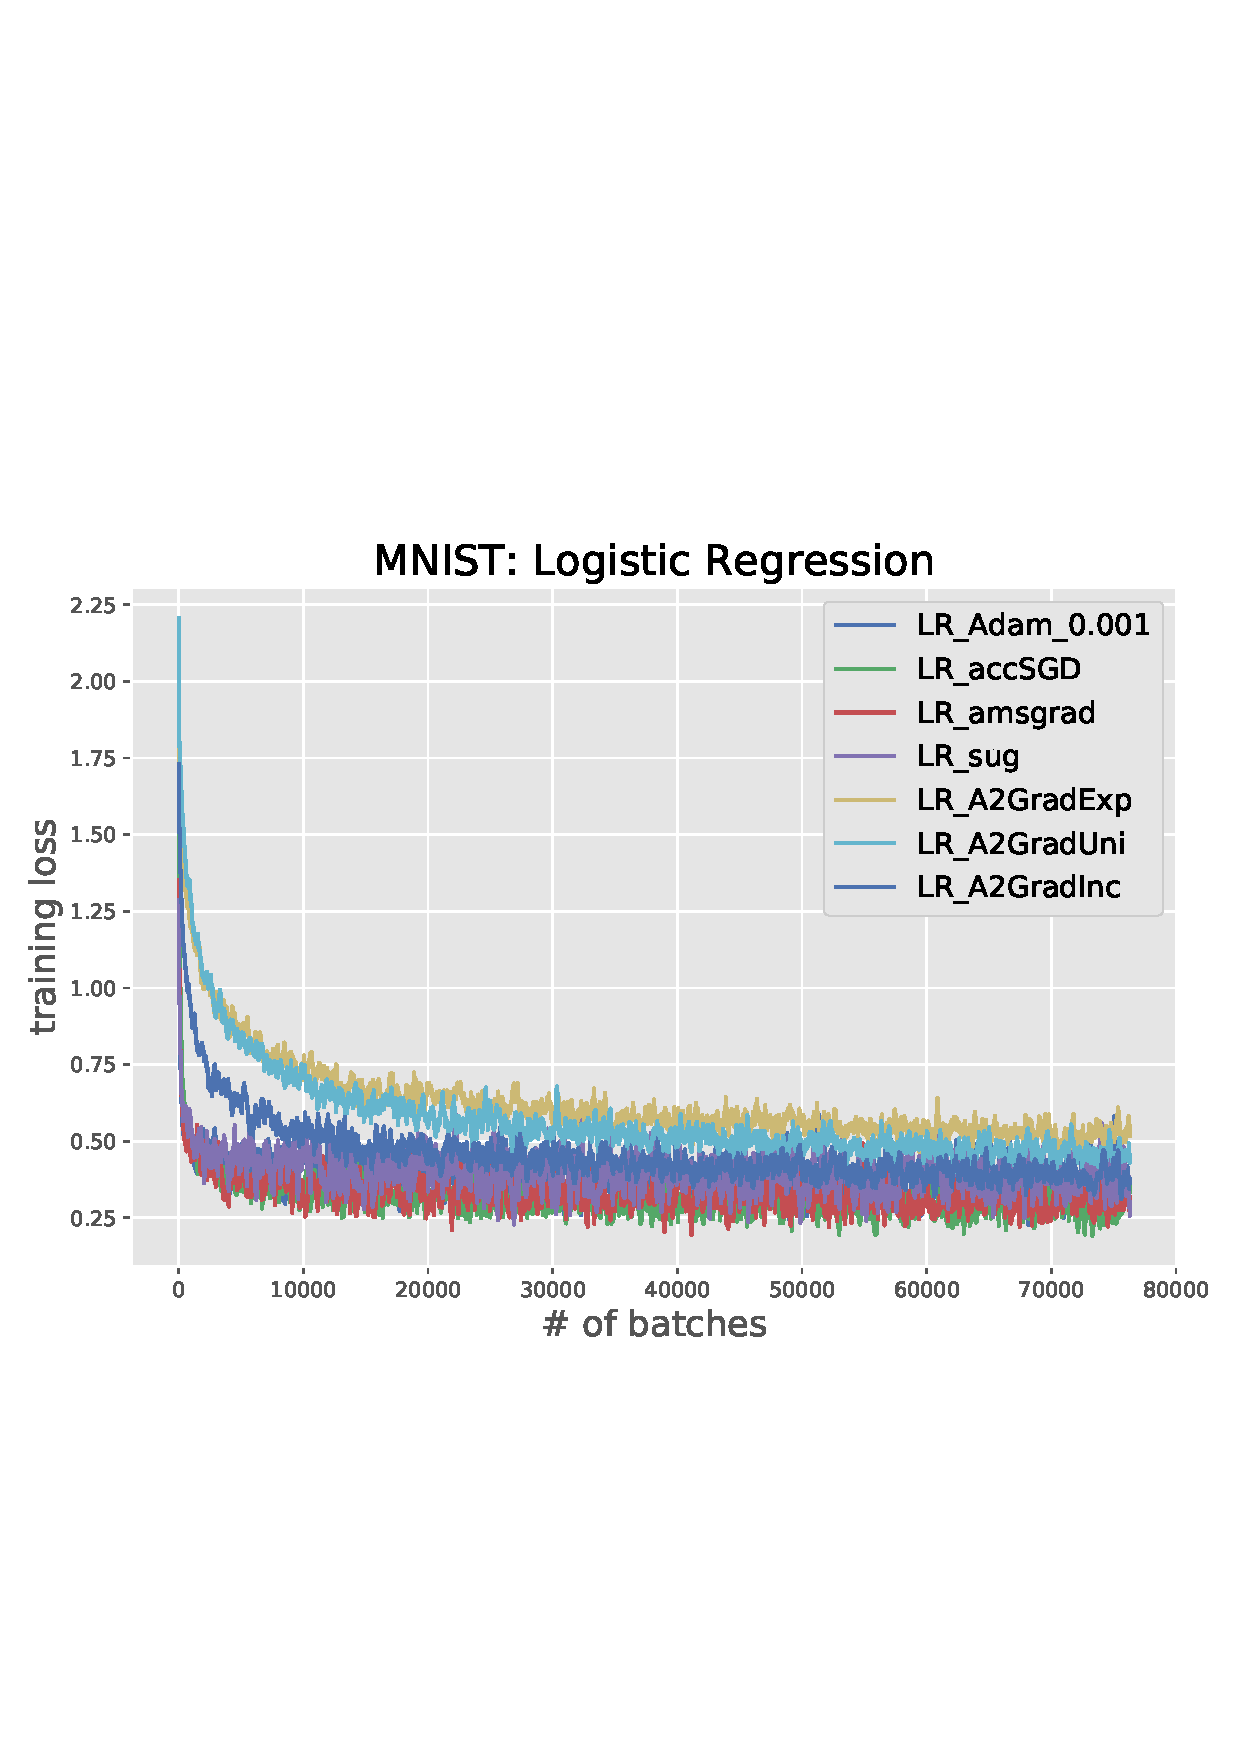
\includegraphics[width=\linewidth]{mnist_logreg_bt.png}
		\endminipage\hfill
		\minipage{0.32\textwidth}
		\includegraphics[width=\linewidth]{mnist_logreg_ep.png}
		\endminipage\hfill
		\minipage{0.32\textwidth}%
		\includegraphics[width=\linewidth]{mnist_logreg_val_ep.png}
		\endminipage
	\end{figure}
	
	\begin{figure}[!htb]
		\minipage{0.32\textwidth}
		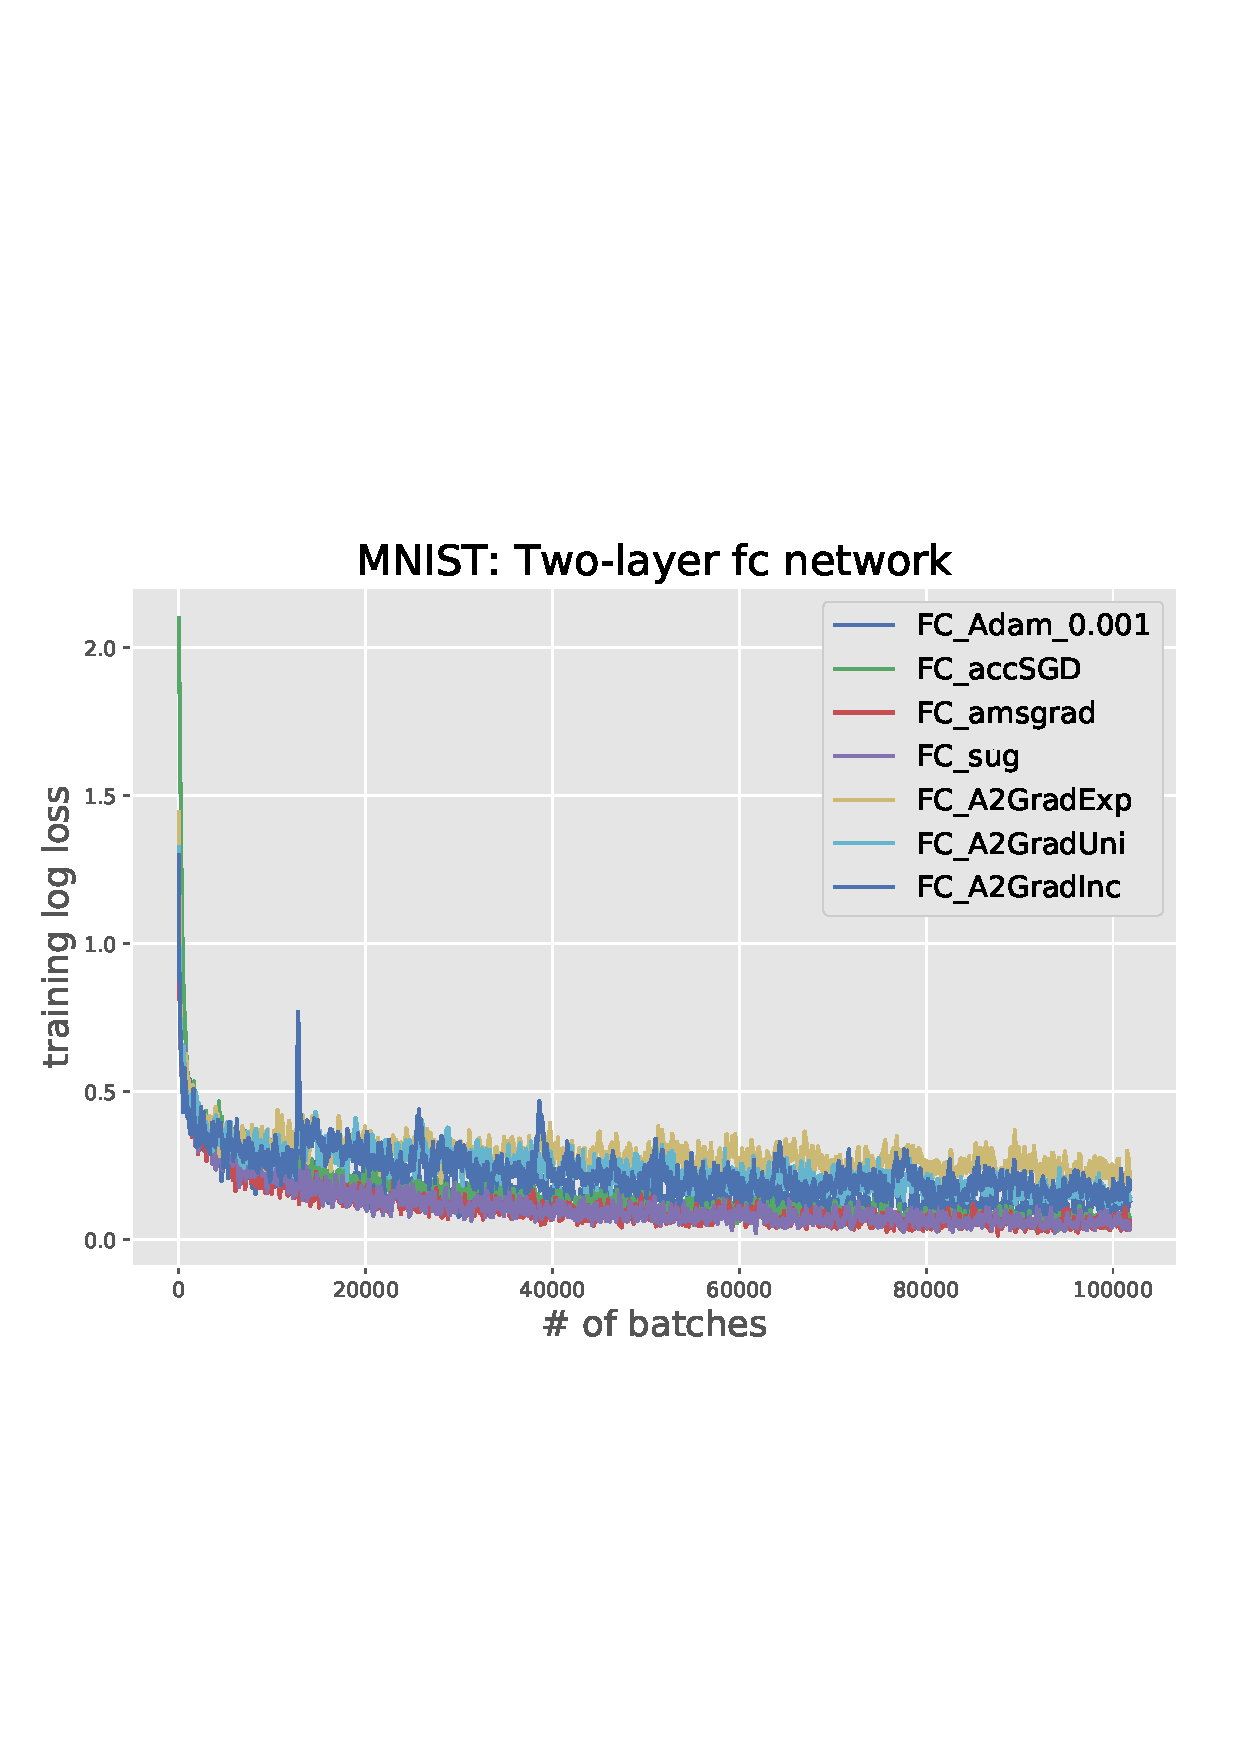
\includegraphics[width=\linewidth]{mnist_fc_bt.png}
		\endminipage\hfill
		\minipage{0.32\textwidth}
		\includegraphics[width=\linewidth]{mnist_fc_ep.png}
		\endminipage\hfill
		\minipage{0.32\textwidth}%
		\includegraphics[width=\linewidth]{mnist_fc_val.png}
		\endminipage
	\end{figure}
	
	\begin{figure}[!htb]
		\minipage{0.32\textwidth}
		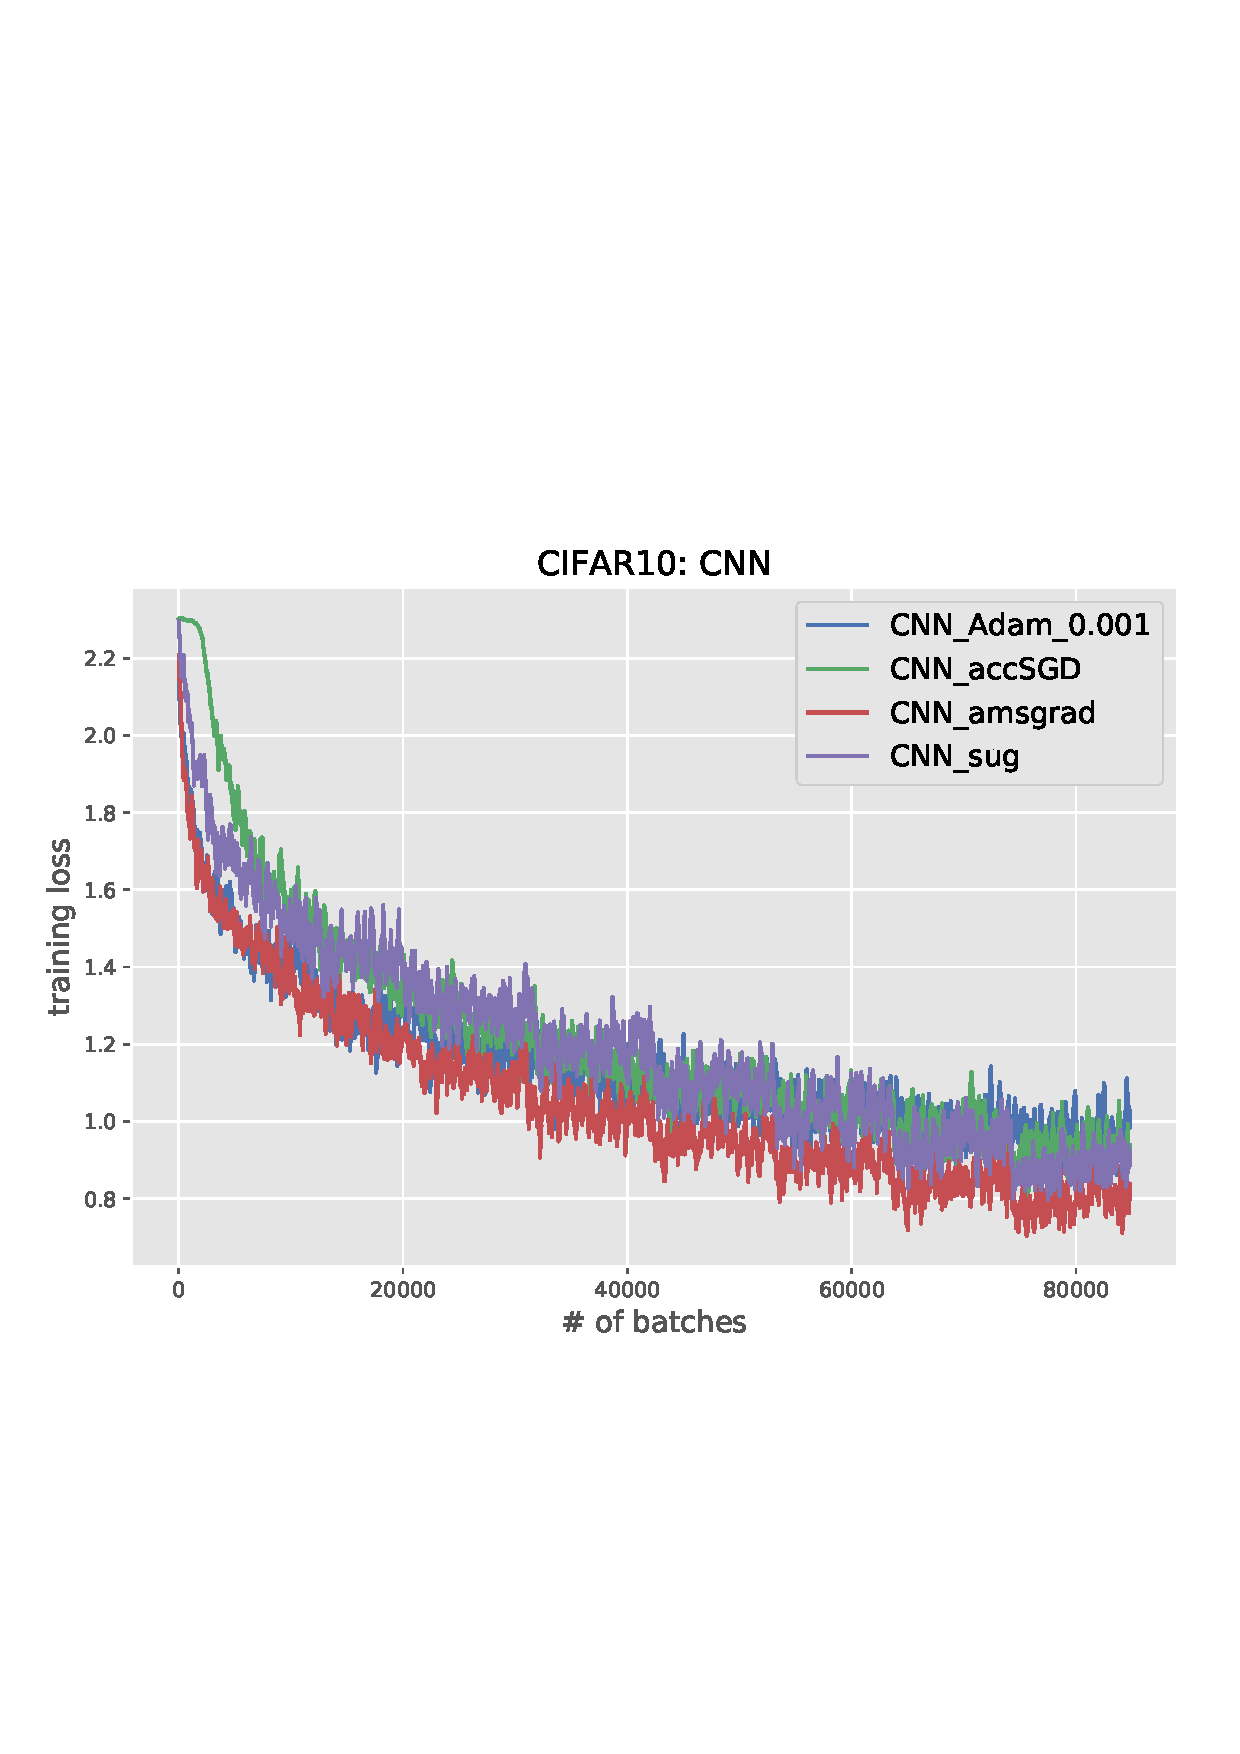
\includegraphics[width=\linewidth]{cifar_cnn_bt.png}
		\endminipage\hfill
		\minipage{0.32\textwidth}
		\includegraphics[width=\linewidth]{cifar_cnn_ep.png}
		\endminipage\hfill
		\minipage{0.32\textwidth}%
		\includegraphics[width=\linewidth]{cifar_cnn_val.png}
		\endminipage
		\caption{Первый ряд графиков показывает результаты эксперимента для Logistic Regression на датасете MNIST. Второй - two-layer neural network тоже на MNIST. Последний ряд показывает результаты работы CNN на датасете CIFAR10.}
	\end{figure}
	
	
	
	\section{Заключение}
	В данной работе был реализован алгоритм $A2Grad$. Анализ ошибки говорит о том, что этот алгоритм выигрывает в скорости сходимости у всех сравниваемых с ним алгоритмов, но, либо немного хуже, либо показывает такие же результаты в самой сходимости.
	
	\newpage
	
	\begin{thebibliography}{4} 
		\bibitem{gas} \textit{Гасников А.В.} Современные численные методы оптимизации. Метод универсального градиентного спуска
		
		\bibitem{seminar} \textit{Камзолов Д.И.} Семинары 674 группы 
		
		\bibitem{lectures} \textit{Камзолов Д.И.} Лекции ФИВТ
		
		\bibitem{presentation} \textit{Камзолов Д.И.} Презентации 674 группы
		
		\bibitem{india} \textit{Rahul Kidambi, Praneeth Netrapalli, Prateek Jain, Sham M. Kakade,} On the insufficiency of existing momentum schemes for Stochastic Optimization
		
		\bibitem{china} \textit{Qi Deng, Yi Cheng, Guanghui Lan,} Optimal Adaptive and Accelerated Stochastic Gradient Descent
		
	\end{thebibliography}
	
	
\end{document} 	